% Ejemplo de documento LaTeX
% Tipo de documento y tamaño de letra
\documentclass[10pt]{article}
% Preparando para documento en Español.
% Para documento en Inglés no hay que hacer esto.
\usepackage[spanish]{babel}
\selectlanguage{spanish}
\usepackage[utf8]{inputenc}


% EL titulo, autor y fecha del documento
\title{Descripción de las prácticas}
\author{Rios Quijada Danira}
\date{20 de Febrero de 2015}
% Aqui comienza el cuerpo del documento
\usepackage{graphicx}
\begin{document}
% Construye el título
\maketitle
\section{Área}
En esta práctica realizamos un programa que calcula el área de un círculo, introduciendole el radio de discho círculo.

\subsection{Código}
\begin{tabular}{l}
\begin{verbatim}  
 Program Circle_area 

   Implicit None 

   Real *8 :: radius , circum , area 

  Real *8 :: PI = 4.0 * atan(1.0) 

   Integer :: model_n = 1 

   print * , 'Enter a radius:' 

   read * , radius !

  circum = 2.0 * PI * radius 

  area = radius * radius * PI 

  print * , 'Program number =' , model_n 

  print * , 'Radius =' , radius 

  print * , 'Circumference =' , circum 
  print * , 'Area =' , area 

 End Program Circle_area
\end{verbatim} \\

\subsection{Compilación}\\

\begin{center}
   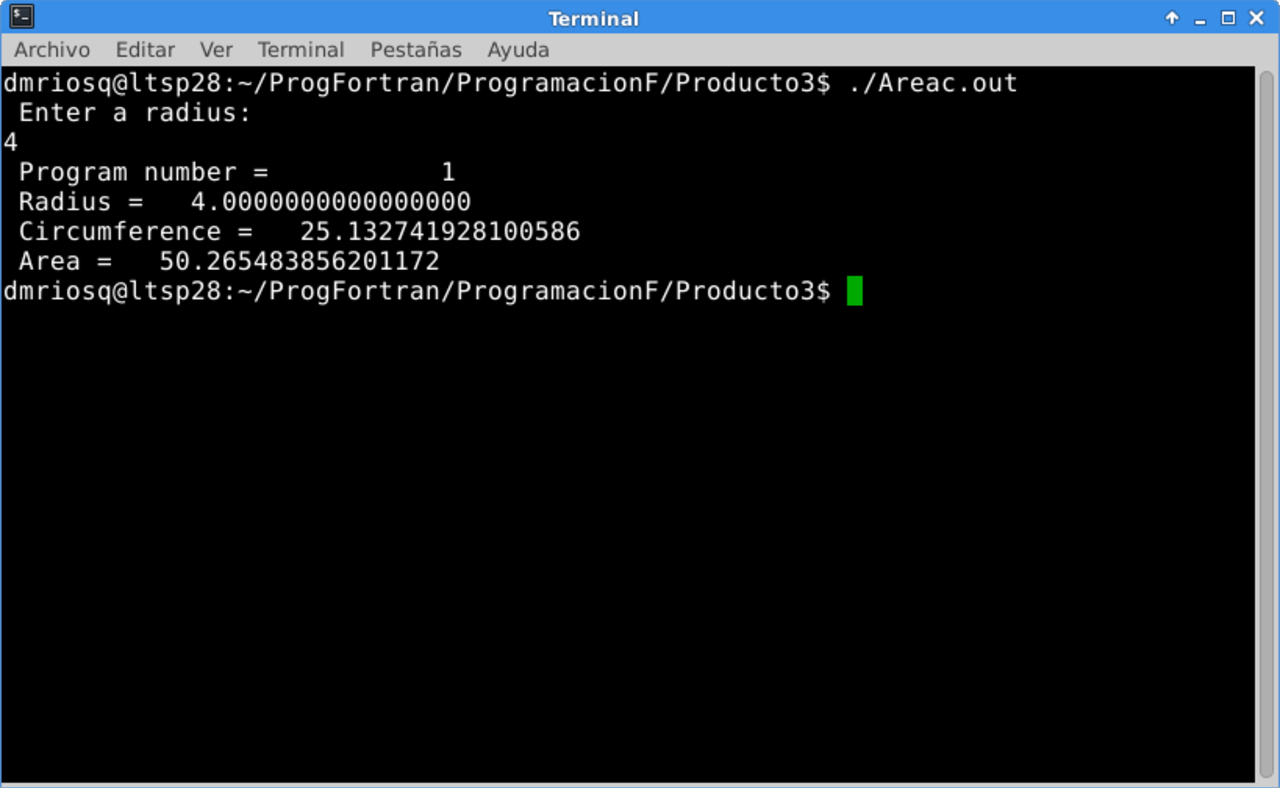
\includegraphics[scale=0.4]{A}
\end{center}
\end{tabular}





\section{Volumen}
En esta práctica realizamos un programa que calcula el volumen de un líquido en un recipiente esférico, dependiendo del radio del recipiente y de la altura a la que se encuentre dicho líquido.


\subsection{Código}
\begin{tabular}{l}
\begin{verbatim}  
 Program Volumen_altura 

   Implicit None 

   Real *8 :: radio , vol , altura 

  Real *8 :: PI = 4.0 * atan(1.0) 

   Integer :: model_n = 2 

   print * , 'Enter a radius:'
read * , radio 
print * , 'Enter a height:'

    
read * , altura

   vol = (PI*(altura*altura))*(radio-(altura/3))

  print * , 'Program number =' , model_n 

  print * , 'Radius =' , radio 
 print * , 'Height=' , altura
   
  print * , 'Volumen =' , vol 

 End Program Volumen_altura
\end{verbatim} \\
\subsection{Compilación}\\

\begin{center}
   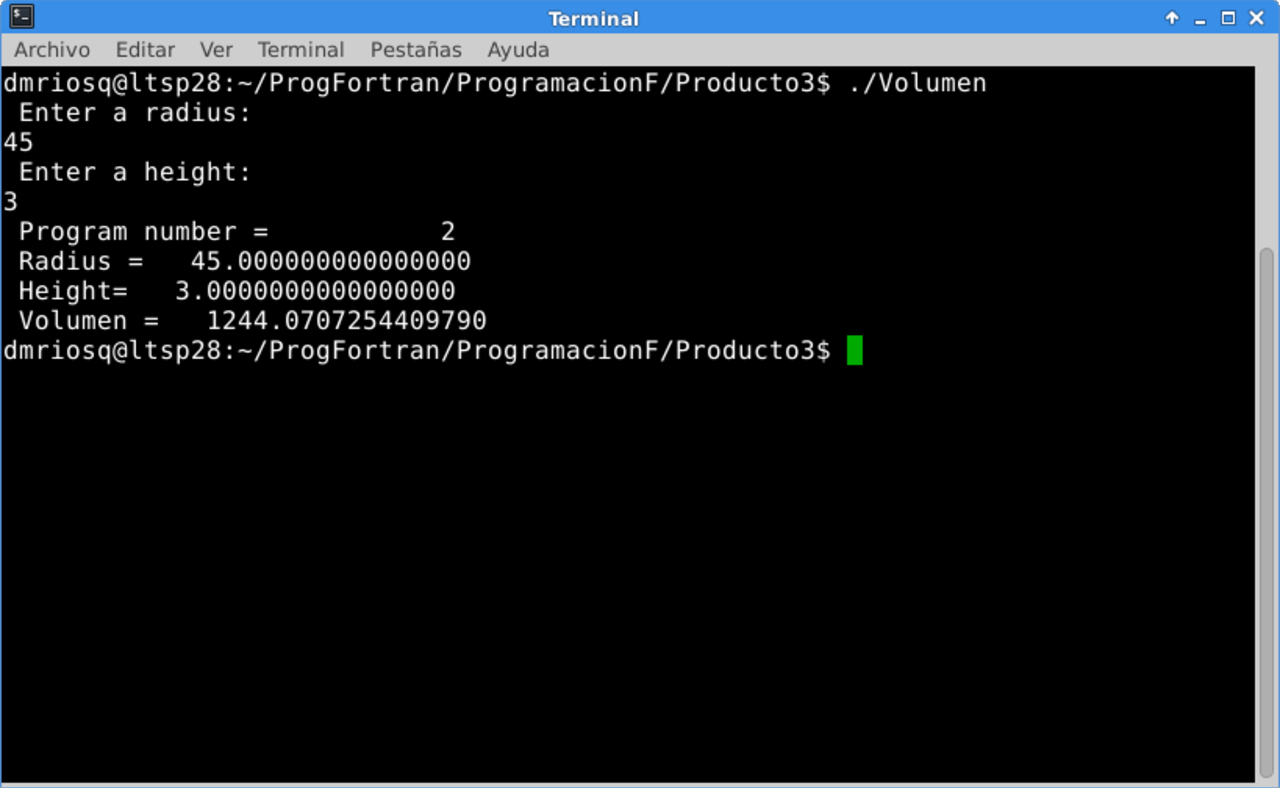
\includegraphics[scale=0.4]{V}
\end{center}
\end{tabular}






\section{Limites}
En esta práctica realizamos un programa que determina la precisión de la maquina en la que se esta ejecutando el programa.

\subsection{Código}
\begin{tabular}{l}
\begin{verbatim}  
  ! Limits . f90 : Determines machine precision

 ! −−−−−−−−−−−−−−−−−−−−−−−−−−−−−

 Program Limits

   Implicit None

   Integer :: i , n

   Real * 4 :: epsilon_m , one
   n=60 ! Establish the number of iterations

  ! Set initial values :
   epsilon_m = 1.0

  one = 1.0

  ! Within a DO−LOOP, calculate each step and print .

  ! This loop will execute 60 times in a row as i is

 ! incremented from 1 to n ( since n = 60) :

  do i = 1, n , 1 ! Begin the do−loop

    epsilon_m = epsilon_m / 2.0 ! Reduce epsilon m

    one = 1.0 + epsilon_m ! Re−calculate one

    print * , i , one , epsilon_m ! Print values so far

  end do ! End loop when i>n
\end{verbatim} \\
\subsection{Compilación}\\

\begin{center}
   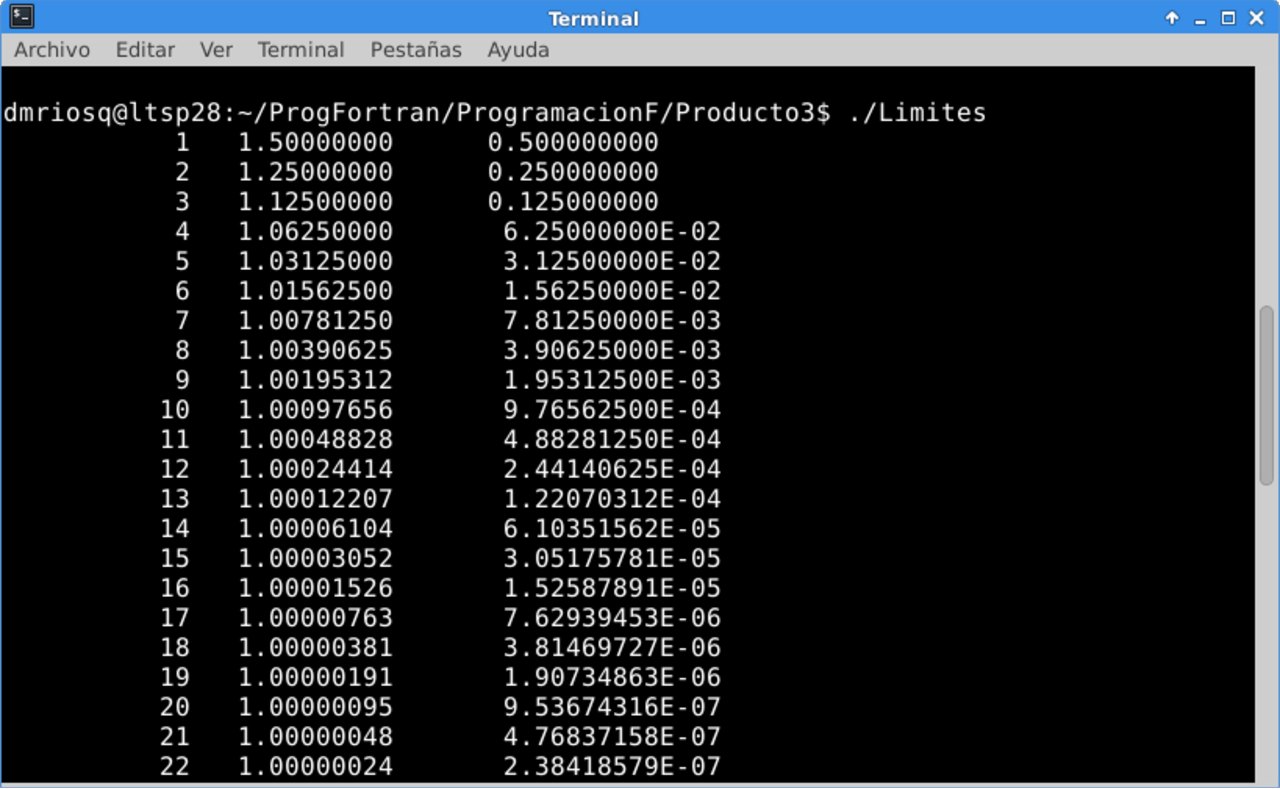
\includegraphics[scale=0.4]{L}
\end{center}
\end{tabular}






\section{Math}
En esta práctica realizamos un programa que calcula la raíz cuadrada real de -1, la arctan de 2 y el log de 0, los cuales son valores indefinidos o inexistentes en los reales.

\subsection{Código}
\begin{tabular}{l}
\begin{verbatim}  
 ! Math . f90 : demo some Fortran math functions

 ! −−−−−−−−−−−−−−−−−−−−−−−−−−−−−−−−−−−−−−−−−−

 Program Math_test ! Begin main program

  Real *8 :: i, p, x = -1.0 , y = 0, z = 2.0, w ! Declare variables x, y, z

 
   i = SQRT (x) ! Call the sine function

   p = LOG (y)  ! Call the exponential function
   w= ASIN (z)

  print * , i, p, w ! Print x, y, z

 End Program Math_test ! End main program 
\end{verbatim} \\
\subsection{Compilación}\\

\begin{center}
   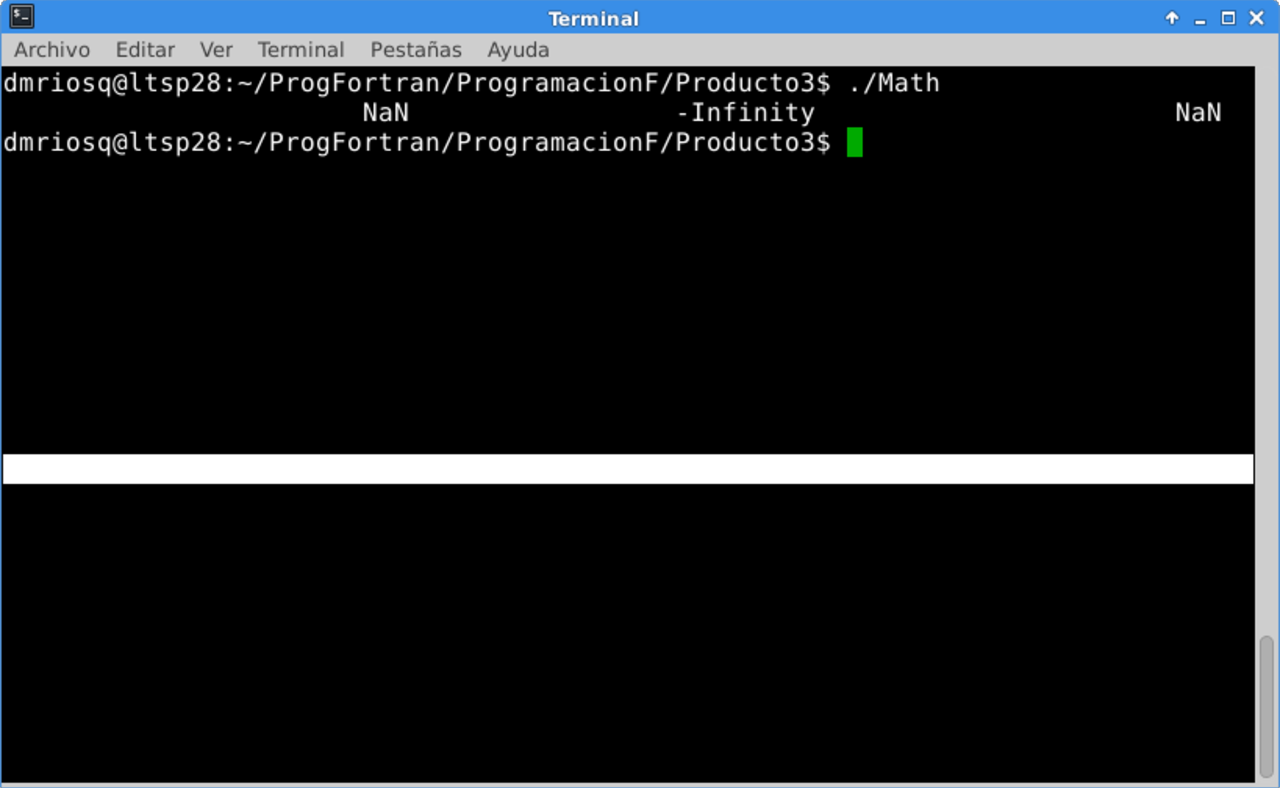
\includegraphics[scale=0.4]{M}
\end{center}
\end{tabular}






\section{Funciones}
En esta práctica realizamos un programa que calcula el valor de una función de 2 variables.

\subsection{Código}
\begin{tabular}{l}
\begin{verbatim}  
 ! Function . f90 : Program calls a simple function

 ! −−−−−−−−−−−−−−−−−−−−−−−−−−−−−−−

 Real *8  Function f (x,y)

   Implicit None

   Real *8 :: x, y

   f = 1.0 + sin(x*y)

 End Function f



 Program Main

  Implicit None

  Real *8 :: Xin =0.25 , Yin =2. , c , f ! declarations ( also f)

  c = f ( Xin , Yin )

 write ( * , * ) 'f(Xin, Yin) =' , c

 End Program Main 
\end{verbatim} \\
\subsection{Compilación}\\

\begin{center}
   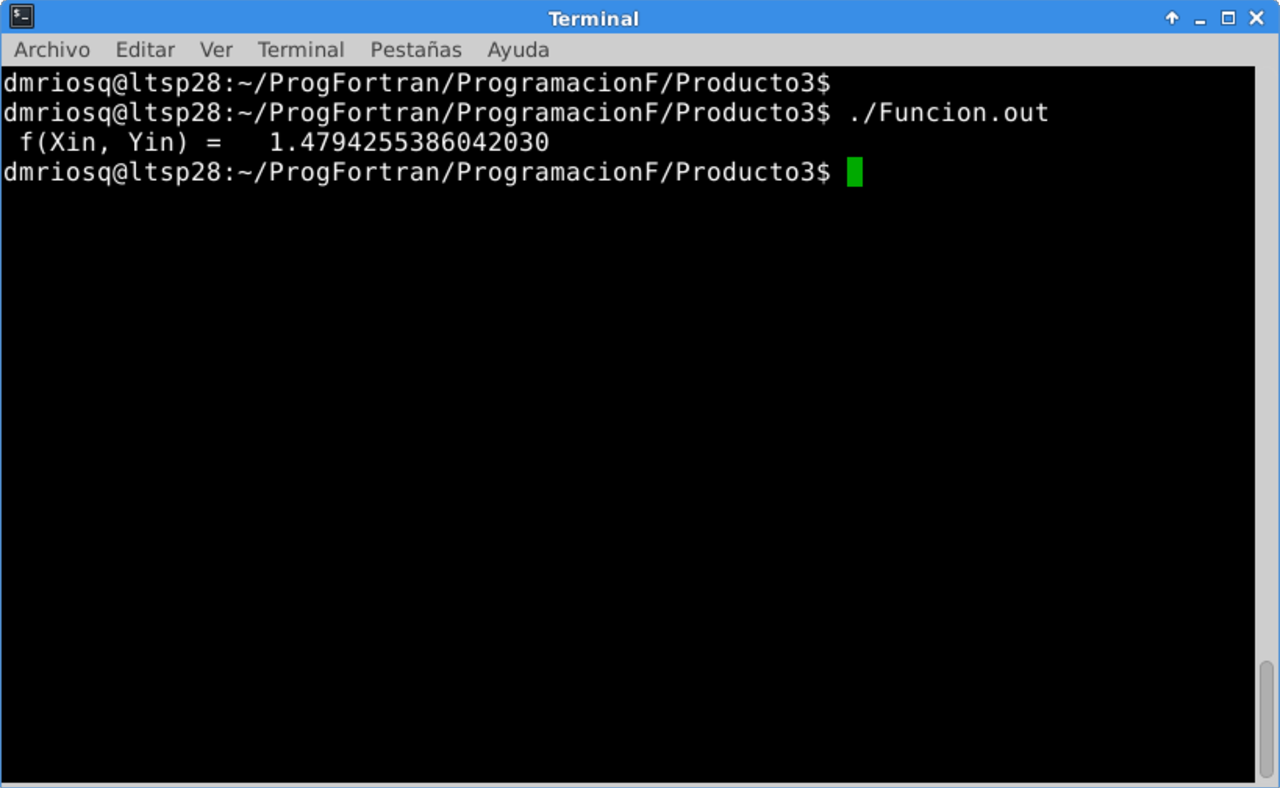
\includegraphics[scale=0.4]{F}
\end{center}
\end{tabular}






\section{Subrutina}
En esta práctica realizamos una subrutina, el cual es un subproceso, que forma parte de un proceso principal.
\subsection{Código}
\begin{tabular}{l}
 \begin{verbatim}  
 ! Subroutine . f90 : Demonstrates the call for a simple subroutine

 ! −−−−−−−−−−−−−−−−−−−−−−−−−−−−−−−−−−−−−−−−−−−−−

 Subroutine g(x, y, ans1 , ans2 )

   Implicit None

   Real (8) :: x , y , ans1 , ans2 ! Declare variables

   ans1 = sin (x*y) + 1. ! Use sine intrinsic func.

   ans2 = ans1**2

 End Subroutine g

 !

 Program Main  

   Implicit None

   Real *8 :: Xin =0.25 , Yin =2.0 , Gout1 , Gout2

   call g( Xin , Yin , Gout1 , Gout2 ) ! Call the subr g

   write ( * , *) 'The answers are:' , Gout1 , Gout2

 End Program Main
\end{verbatim} \\
\subsection{Compilación}\\

\begin{center}
   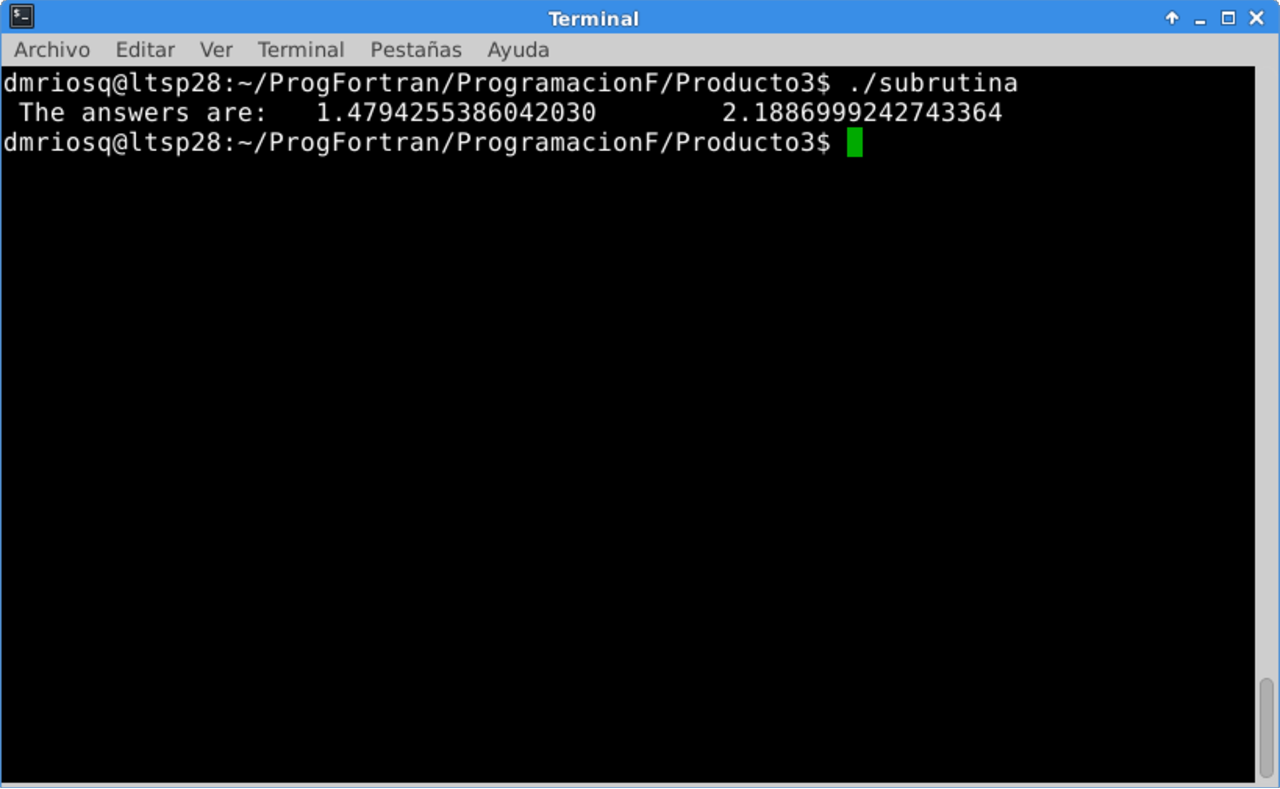
\includegraphics[scale=0.4]{S}
\end{center}
\end{tabular}







% Nunca debe faltar esta última linea.
\end{document}
